\titre{diagramme sagittal} (graphique)
\begin{center}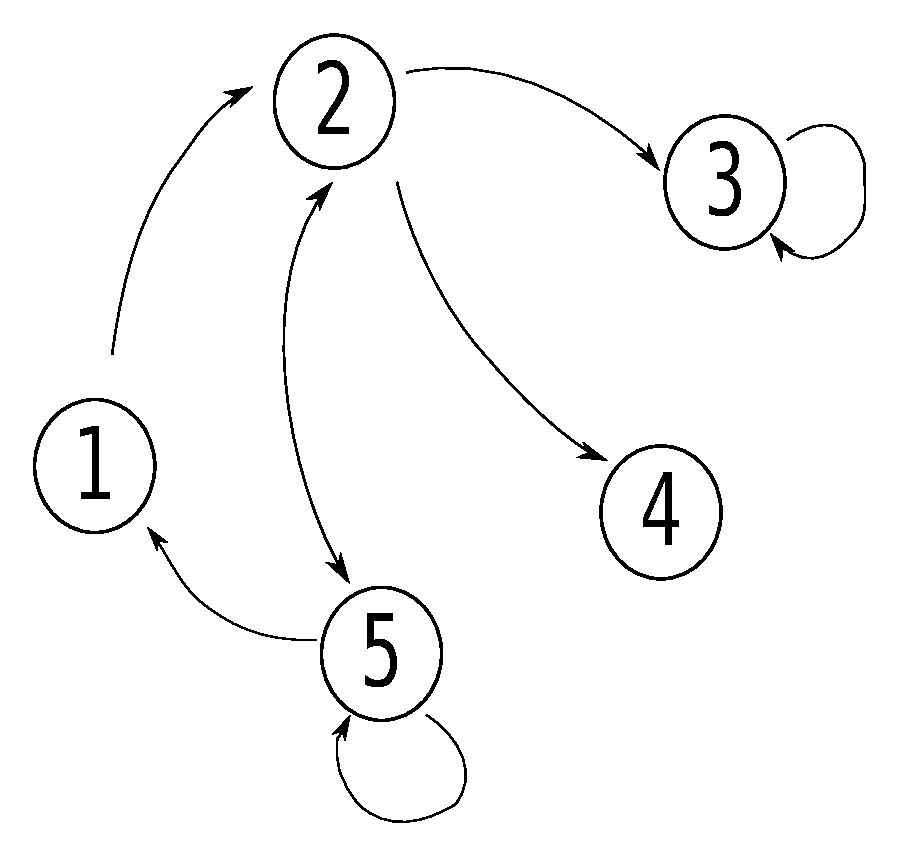
\includegraphics[width=5cm]{D4_1.pdf}\end{center}
\par
\titre{tableau d'attribution des arcs} (matrice booléenne)
$$\left( \begin{array}{ccccc} 
		0 & 1 & 0 & 0 & 0 \\
		0 & 0 & 1 & 1 & 1 \\
		0 & 0 & 1 & 0 & 0 \\
		0 & 0 & 0 & 0 & 0 \\
		1 & 0 & 0 & 0 & 1 
		\end{array} \right)$$

\par

\titre{Dictionnaire des successeurs ou des prédécesseurs}
$$\begin{array}{c|l}
	1 & 2 \\
  2 & 3 ; 4 ; 5 \\
	3 & 3 \\
	4 & \vide \\
	5 & 1 ; 5 \\
\end{array}
\hskip 3cm
\begin{array}{c|l}
	1 & 5 \\
	2 & 1 ; 5 \\
	3 & 2 ; 3 \\
	4 & 2 \\
	5 & 2 ; 5
\end{array}$$ 
